%!TEX root = ../paper.tex

% Small differences in anisotropy  
In \cref{s:results} some differences in anisotropy of the kernels were observed, however these differences were relatively small. This section investigates the anisotropy of the kernels. 
	
		% Single Sphere
			\begin{figure}
				\centering
				\begin{subfigure}{0.23\textwidth}
					\centering
					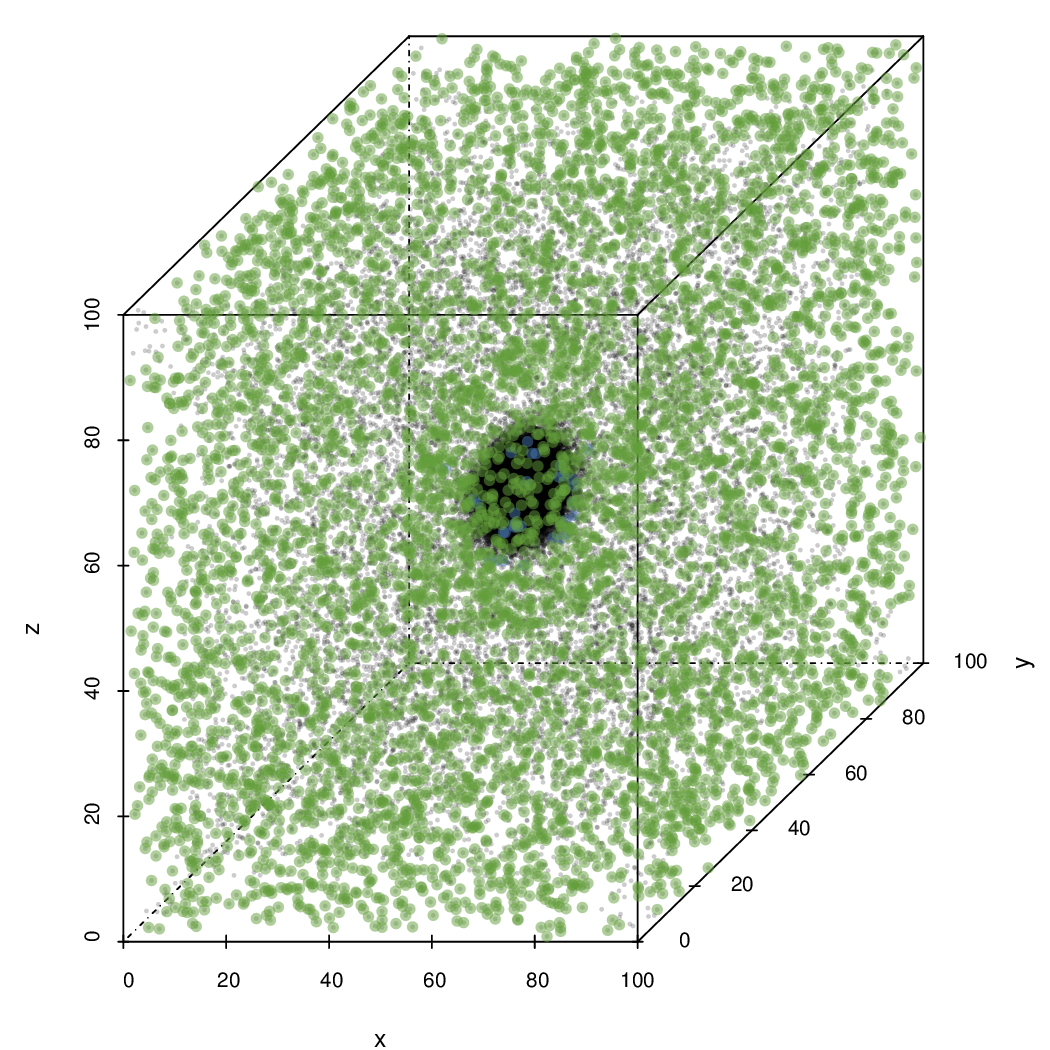
\includegraphics[keepaspectratio=true, width=\textwidth, height=0.23\textheight]{discussion/img/ferdosi_1_60000_anisotropy.png}
					\caption{\ferdosiOne [\num{2.783732800937043e+00}, \num{4.876641609906343e+00}]}
					\label{fig:discussion:anisotropy:ferdosi1}
				\end{subfigure}
				\begin{subfigure}{0.23\textwidth}
					\centering
					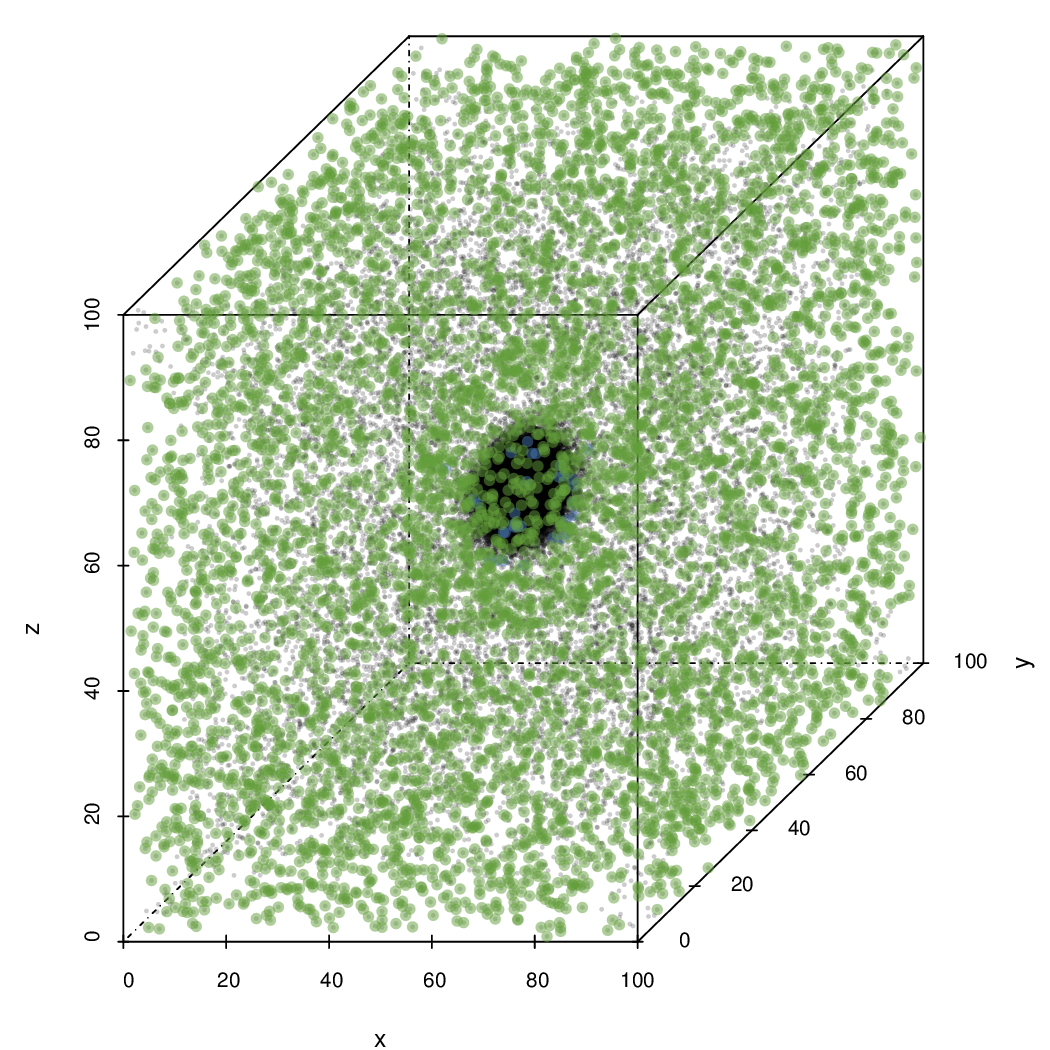
\includegraphics[keepaspectratio=true, width=\textwidth, height=0.23\textheight]{discussion/img/ferdosi_1_60000_anisotropy.png}
					\caption{\baakmanOne [\num{2.955638611296131e+00}, \num{4.876641609906340e+00}]}
					\label{fig:discussion:anisotropy:baakman1}
				\end{subfigure}	
				\begin{subfigure}{0.23\textwidth}
					\centering
					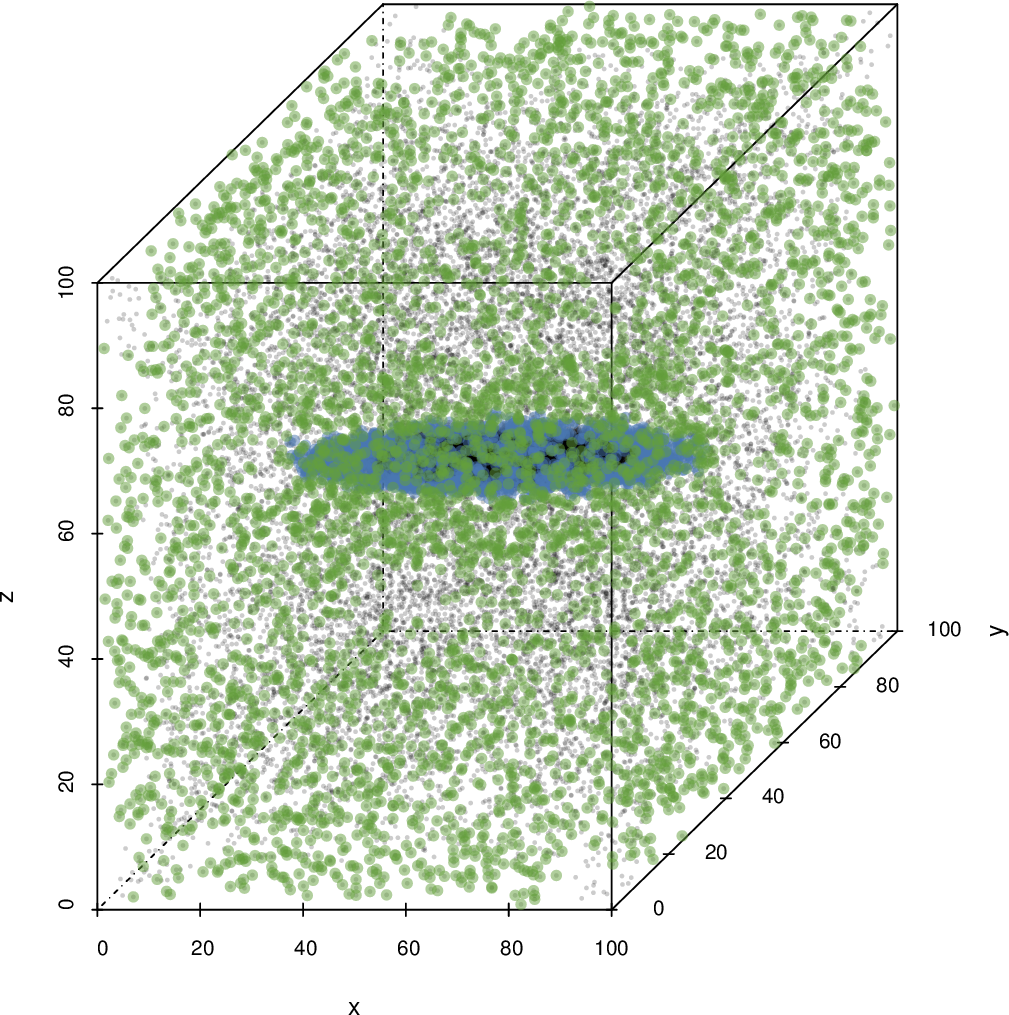
\includegraphics[keepaspectratio=true, width=\textwidth, height=0.23\textheight]{discussion/img/baakman_4_60000_anisotropy.png}
					\caption{\baakmanFour [\num{3.105833113039985e+00}, \num{5.987200775539245e+00}]}
					\label{fig:discussion:anisotropy:baakman4}
				\end{subfigure}		
				\begin{subfigure}{0.23\textwidth}
					\centering
					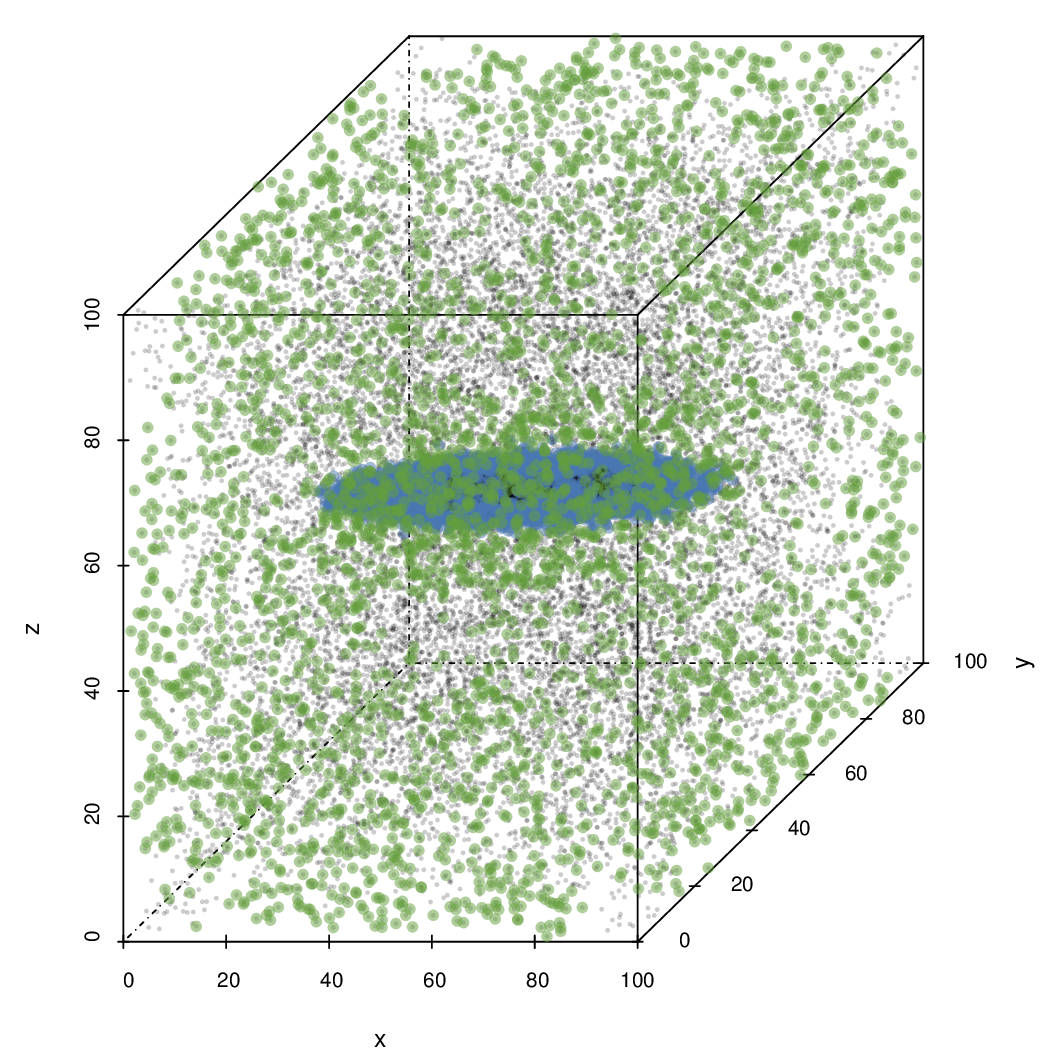
\includegraphics[keepaspectratio=true, width=\textwidth, height=0.23\textheight]{discussion/img/baakman_5_60000_anisotropy.png}
					\caption{\baakmanFive [\num{3.546238846198991e+00}, \num{8.192210308245695e+00}]}
					\label{fig:discussion:anisotropy:baakman5}
				\end{subfigure}			
				\caption{Scatter plot of the data sets
					\subref{fig:discussion:anisotropy:ferdosi1} \ferdosiOne, %
					\subref{fig:discussion:anisotropy:baakman1} \baakmanOne, %
					\subref{fig:discussion:anisotropy:baakman4} \baakmanFour, and %
					\subref{fig:discussion:anisotropy:baakman5} \baakmanFive. %
					The points with kernels whose anisotropy lies in the \nth{90} percentile are shown larger and in the color of the component they were drawn from. The range of the anisotropy of the kernels of the emphasized points in shown below each plot.}
				\label{fig:discussion:anisotropy:singleSphere}
			\end{figure}
			%	
			To that end plot \cref{fig:discussion:anisotropy:singleSphere} shows the datasets with a single Gaussian with points whose anisotropy lies in the \nth{90} percentile emphasized. 
				% Ferdosi 1 & Baakman 1
				In this figure hardly any difference is visible between \cref{fig:discussion:anisotropy:ferdosi1,fig:discussion:anisotropy:baakman1}. 
					% Very few points from Gaussian comonent
					Although it is hardly visible in the plots \percentage{5.180481283422460e-01} and \percentage{1.174799465240642e+01} of the emphasized points are sampled from the Gaussian component of dataset \ferdosiOne and \baakmanOne, respectively. Which illustrates that the kernels in dataset \baakmanOne are influenced by the anisotropy of the Gaussian component of that dataset.
					% Shell of points sampled from the noise around the Gaussian comonent
					Furthermore a shall op points sampled from the noise seems to surround the Gaussian component, it is quite likely that the shape of the kernel of these points is influenced by the Gaussian component. 
					% Explanation: high density -> anisotropy detection fails
					We expect that nearer to the mean of the Gaussian component fewer kernels are influenced by its anisotropy as the physical density of points is quite high in that area. Consequently the volume of the local neighborhood is quite small, and is therefore not representative of the shape of the Gaussian component. 
				% Baakman 4 and 5
				In dataset \baakmanFour and \baakmanFive the number of points with a kernel with a high anisotropy sampled from the Gaussian components is higher than in dataset \ferdosiOne and \baakmanOne, to be exact \percentage{2.190842245989305e+01} and \percentage{4.207887700534759e+01}, respectively. Thus as the anisotropy of the Gaussian component increases more of the kernels near the component adapt their shape more. 
		
		% Multi Sphere
			\begin{figure}
				\centering
				\begin{subfigure}{0.23\textwidth}
					\centering
					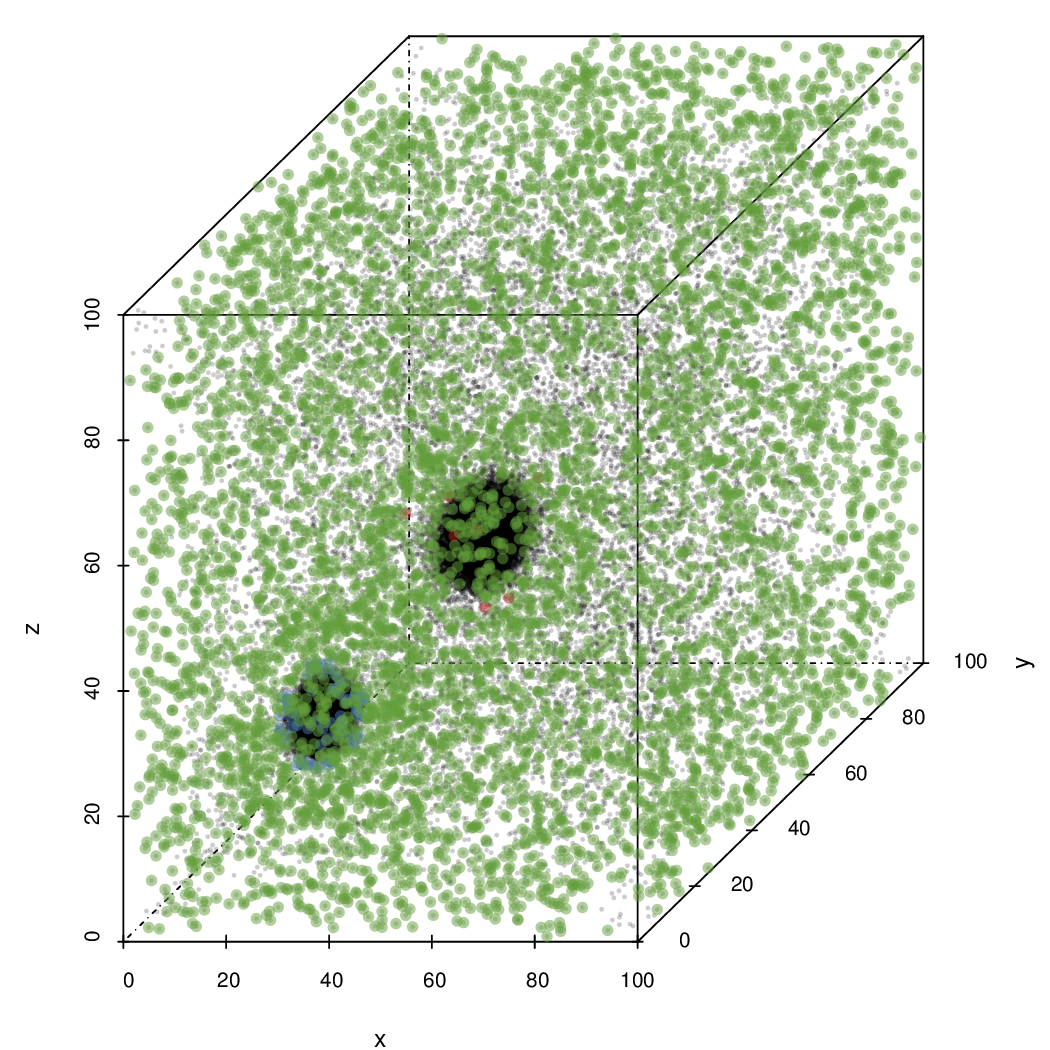
\includegraphics[keepaspectratio=true, width=\textwidth, height=0.23\textheight]{discussion/img/ferdosi_2_60000_anisotropy.png}
					\caption{\ferdosiTwo [\num{2.215970619635167e+00}, \num{5.678002691654005e+00}]}
					\label{fig:discussion:anisotropy:ferdosi2}
				\end{subfigure}
				\begin{subfigure}{0.23\textwidth}
					\centering
					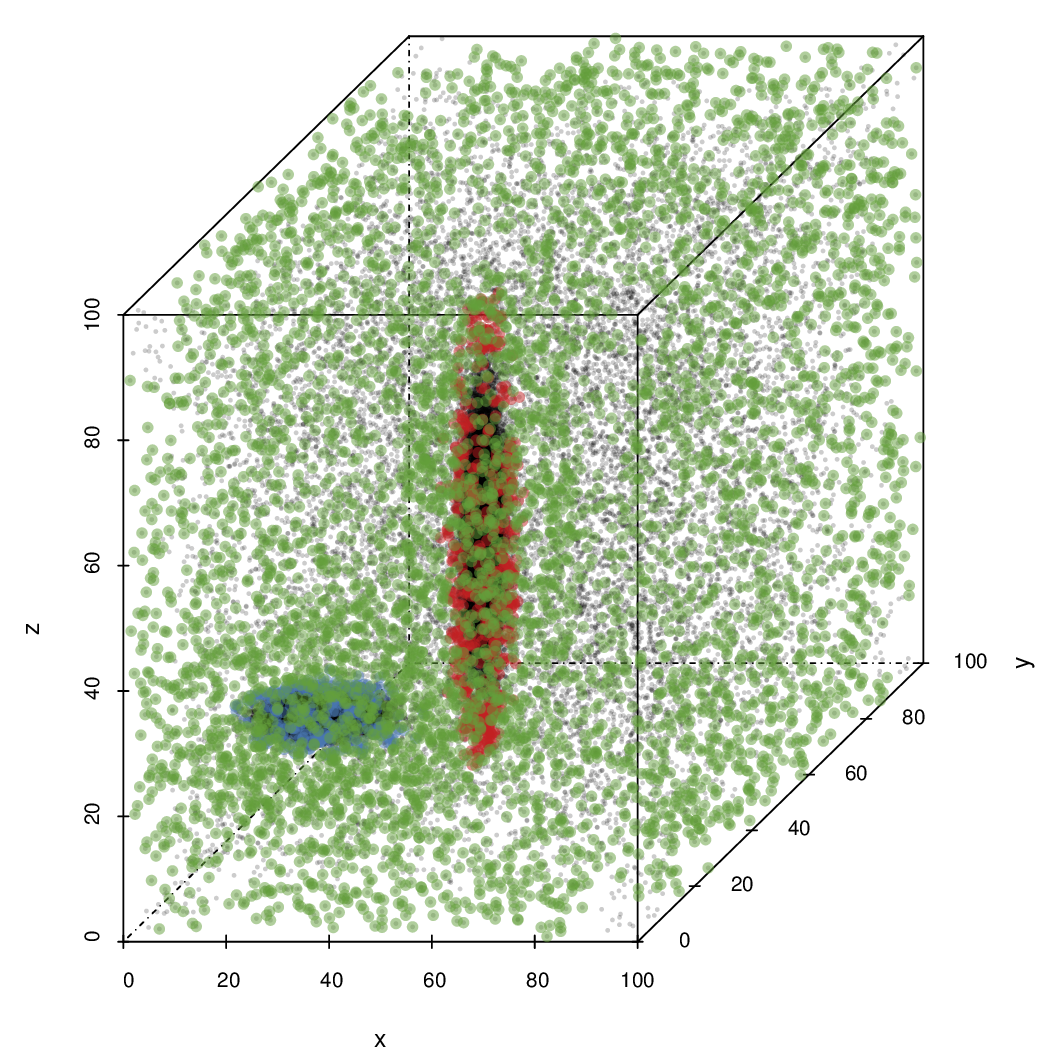
\includegraphics[keepaspectratio=true, width=\textwidth, height=0.23\textheight]{discussion/img/baakman_2_60000_anisotropy.png}
					\caption{\baakmanTwo [\num{2.463414286522871e+00}, \num{7.134567710248723e+00}]}
					\label{fig:discussion:anisotropy:baakman2}
				\end{subfigure}	
				\begin{subfigure}{0.23\textwidth}
					\centering
					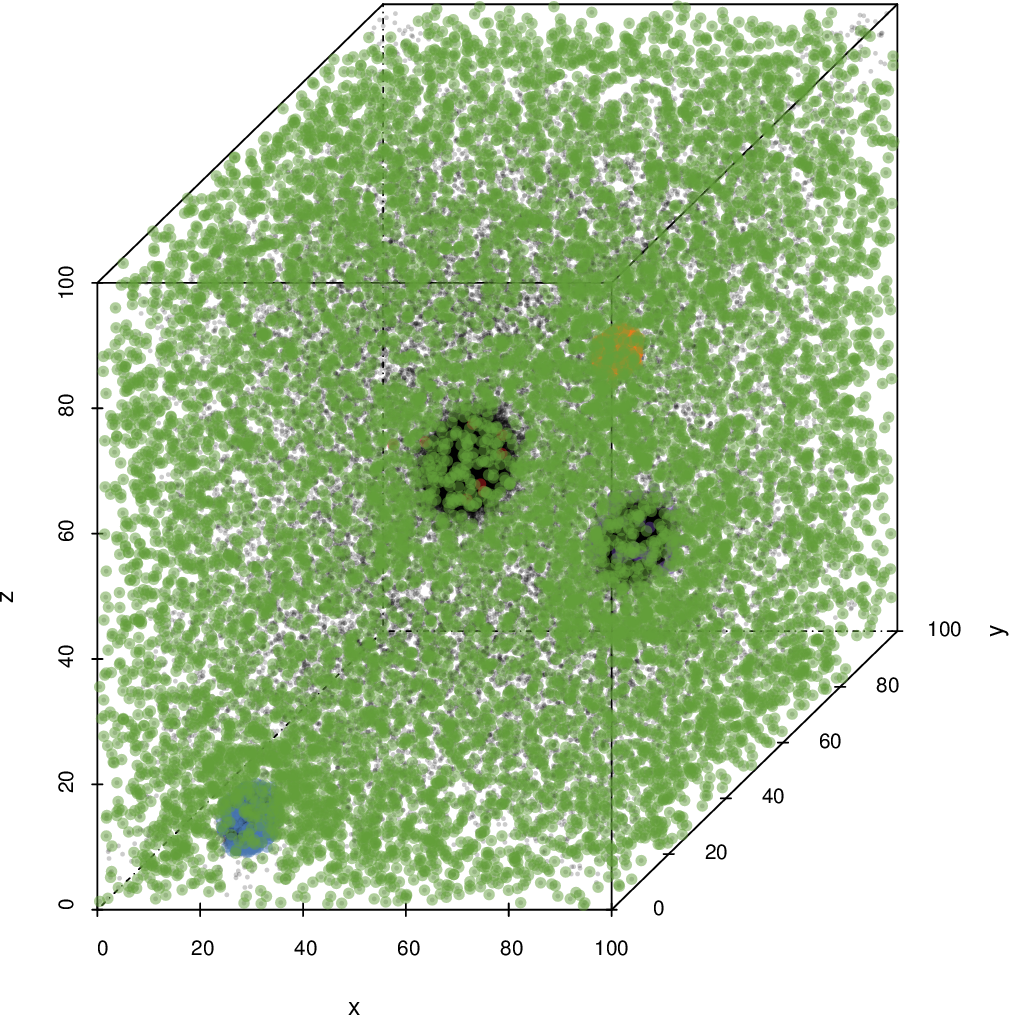
\includegraphics[keepaspectratio=true, width=\textwidth, height=0.23\textheight]{discussion/img/ferdosi_3_120000_anisotropy.png}
					\caption{\ferdosiThree [\num{2.138909227329211e+00}, \num{8.855946762727447e+00}]}
					\label{fig:discussion:anisotropy:ferdosi3}
				\end{subfigure}		
				\begin{subfigure}{0.23\textwidth}
					\centering
					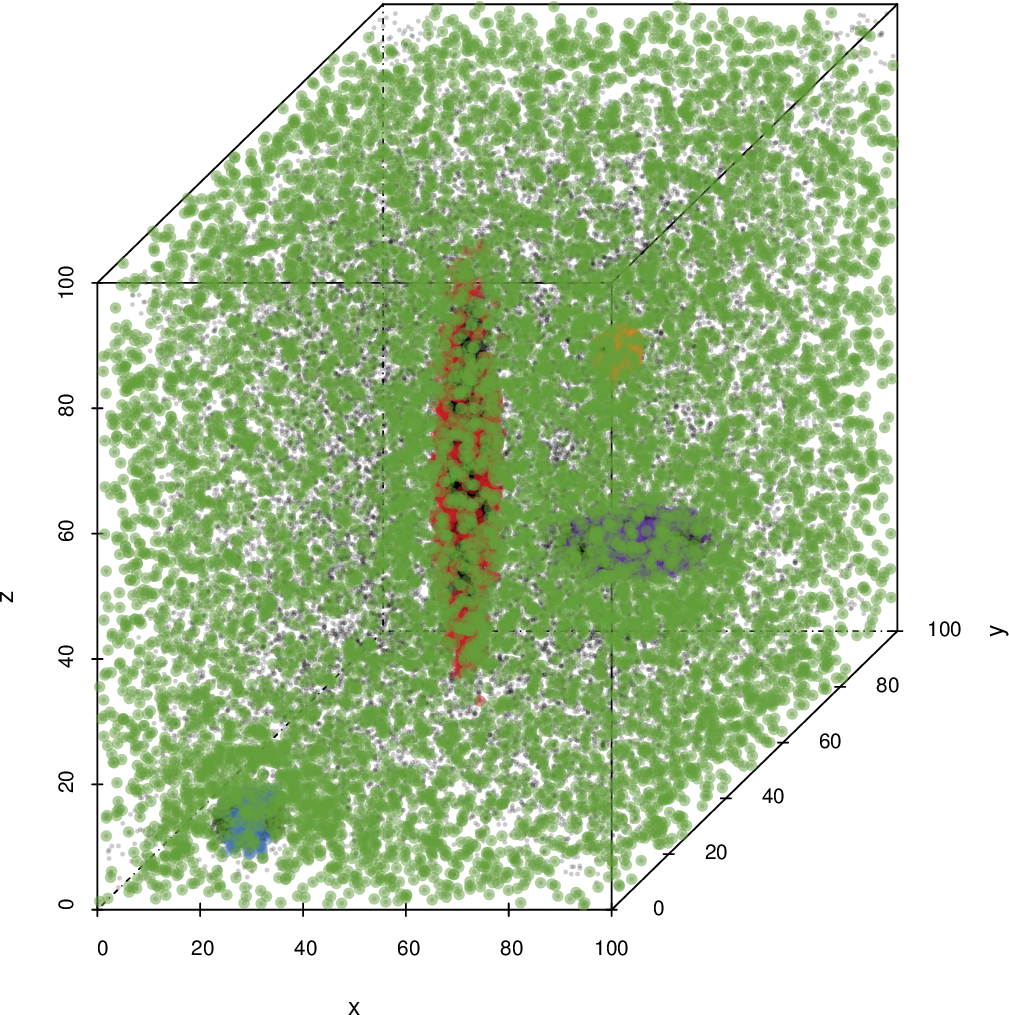
\includegraphics[keepaspectratio=true, width=\textwidth, height=0.23\textheight]{discussion/img/baakman_3_60000_anisotropy.png}
					\caption{\baakmanThree [\num{2.316497642958064e+00}, \num{8.855946762727445e+00}]}
					\label{fig:discussion:anisotropy:baakman3}
				\end{subfigure}			
				\caption{Scatter plot of datasets
					\subref{fig:discussion:anisotropy:ferdosi2} \ferdosiTwo, %
					\subref{fig:discussion:anisotropy:baakman2} \baakmanTwo, %
					\subref{fig:discussion:anisotropy:ferdosi3} \ferdosiThree, and %
					\subref{fig:discussion:anisotropy:baakman3} \baakmanThree. %
					The points that have an anisotropy in the \nth{90} percentile are shown larger and in the color of the component they were drawn from. The range of the anisotropy of the kernels of the emphasized points in shown below each plot.}
				\label{fig:discussion:anisotropy:multisphere}
			\end{figure}			
			% General Introduction
			\Cref{fig:discussion:anisotropy:multisphere} emphasizes the points with the most anisotropic kernels in the dataset \ferdosiTwo through \baakmanThree. 
			% Ferdosi 2
				% Same observations as for ferdosi 1, present percentages
				In the plot associated with dataset \ferdosiTwo we observe the same shells of high anisotropy kernels of points sampled from the noise around the Gaussian components as in dataset \ferdosiOne. Another similarity between these two datasets is that very few points sampled from the Gaussian component have a kernel with high anisotropy; \percentage{1.453877} and \percentage{0.1169786} of the first and second Gaussian component, respectively. 
				% F2G1 vs F2G2
				We contribute the difference in the number of highly anisotropic kernels associated with data points sampled from the two Gaussian components to the difference in density between the two Gaussian components.

			% Baakman 2
				% More points near the Gaussian anisotropic

			% Ferdosi 3
				% G1 and G3 have anisotropic kernels. 

				% Present percentages

				% Relate to results?

				% Why G1 and G3 and not G2 and G4? 
					% G1/G3 are placed near the  border of the dataset, contrast with results of F3Noise?

					% G1/G3 have lower covariance:

			% Baakman 3
				% Any difference between G1/G3 and G2/G4?

		% Some general conclusion
		Lastly in all datasets a large number of points sampled from the background have a high anisotropy. We expect that this is caused by fine structures in the noise that overwhelm the local neighborhood.

% Denser component -> higher anisotropy of kernels
% AND Higher anistropy in component -> higer anisotropy in associated kernels
% AND Denser comonent -> lower MSE
	% Introduce the dataset A1 and A2, same anisotropy different density, what do we observe, what does it say about this correlation.
% Refer back to the difference between G1/G3 versus G2/G4 in F3.

% Lack of difference in anisotropy between F3 and B3 in orange (‘Trivariate Gaussian 3’) component. 

% Some conclusion